\documentclass{standalone}
\usepackage{amsmath}
\usepackage{tikz}

\begin{document}

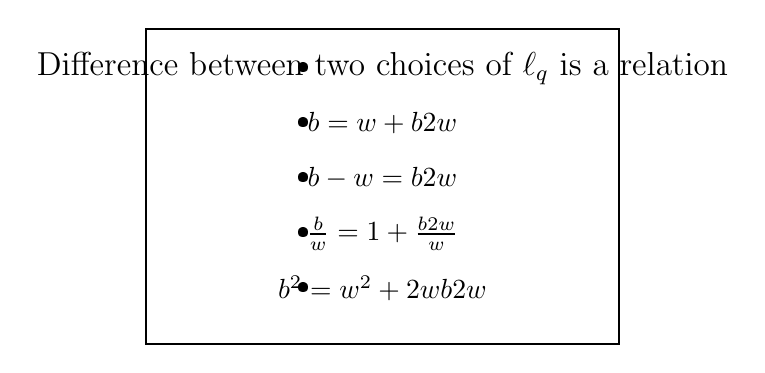
\begin{tikzpicture}[x=1cm, y=1cm]

% Draw the whiteboard frame
\draw[thick] (0,0) rectangle (6,4);

% Add text and equations inside the whiteboard
\node at (3,3.5) [font=\large] {Difference between two choices of $\ell_q$ is a relation};
\node at (3,2.8) {$b = w + b2w$};
\node at (3,2.1) {$b - w = b2w$};
\node at (3,1.4) {$\frac{b}{w} = 1 + \frac{b2w}{w}$};
\node at (3,0.7) {$b^2 = w^2 + 2wb2w$};

% Add additional symbols and notations
\node at (2,3.5) {\textbullet};
\node at (2,2.8) {\textbullet};
\node at (2,2.1) {\textbullet};
\node at (2,1.4) {\textbullet};
\node at (2,0.7) {\textbullet};

\end{tikzpicture}

\end{document}